\documentclass[12pt]{article}
\usepackage{amsmath, amssymb, amsfonts, amsthm}
\usepackage{tikz}
\usetikzlibrary{shapes,calc}
\usetikzlibrary{arrows,automata}

\begin{document}

\begin{figure}[h]
    \centering
    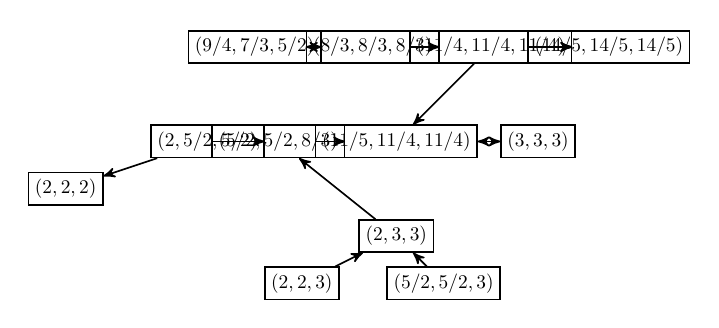
\begin{tikzpicture}[->,>=stealth',auto,node distance=3cm,
                    semithick,scale=0.6, every node/.style={scale=0.7}]
\node[draw] (A) at (-3, -1) {$(2,2,2)$};
\node[draw] (B) at (0, 0) {$(2,5/2,5/2)$};
\node[draw] (C) at (1.5, 0) {$(5/2,5/2,8/3)$};
\node[draw] (D) at (4, 0) {$(11/5,11/4,11/4)$};
\node[draw] (E) at (7, 0) {$(3,3,3)$};
\node[draw] (F) at (4, -2) {$(2,3,3)$};
\node[draw] (G) at (2,-3) {$(2,2,3)$};
\node[draw] (H) at (5, -3) {$(5/2,5/2,3)$};

\node[draw] (I) at (1, 2) {$(9/4,7/3,5/2)$};
\node[draw] (J) at (3.5, 2) {$(8/3,8/3,8/3)$};
\node[draw] (K) at (6, 2) {$(11/4,11/4,11/4)$};
\node[draw] (L) at (8.5, 2) {$(14/5,14/5,14/5)$};

\path[every node/.style={font=\sffamily\small}]
(E) edge node [left] {} (D)
(C) edge node [left] {} (B)
(F) edge node [right] {} (C)
(B) edge node [left] {} (A)
(G) edge node [right] {} (F)
(D) edge node [right] {} (C)
(K) edge node [right] {} (J)
(L) edge node [right] {} (K)
(H) edge node [right] {} (F)
(I) edge node [above] {} (J)
(J) edge node [above] {} (I)
(K) edge node [above] {} (D)
(L) edge node [above] {} (K)
(D) edge node [above] {} (E);
    \end{tikzpicture}
    \caption{Hasse diagram of the poset of discontinuity points of \autoref{th:discont}. Here $u \tikzto v$ means $u \leq v$, and by definition we have $u \leq v$ if there is a permutation of $u$ that is pointwise at most $v$.}
    \label{fig:hasse_diagram_discont}
\end{figure}

\end{document}